\section{Lösungskonzept}
Dieses Kapitel beinhaltet die Beschreibung der Architektur und wichtiger Komponenten. Es werden die theoretischen Grundlagen der eingesetzten Technologien und Systeme erläutert und warum diese verwendet werden. Nicht Teil dieses Kapitels sind Erläuterungen von Konfigurationen und Code. Dies wird separat im Kapitel «Umsetzung» behandelt.

\subsection{Evaluation der Plattform}
Anhand der Marktsituation und den funkionalen Anforderungen haben wir die Vor- und Nachteile der jeweiligen Plattformen miteinander verglichen und dabei darauf geachtet, welche Kriterien für unsere Lösung von Bedeutung sind.

Wichtige Kriterien:
\begin{itemize}
	\item Nachträgliche Installation möglich
	\item Beliebige Szenarien realisierbar
	\item Herstellerunabhängige Komponenten
	\item Erfüllung der Anforderungen F01 - F05
\end{itemize}

Vernachlässigbare Kriterien:
\begin{itemize}
	\item Optisch ansprechende Integration
	\item Installation ohne Fachkenntnisse
\end{itemize}

\subsubsection{Ergebnis: openHAB} 
Mit openHAB haben wir eine Plattform gefunden, die allen wichtigen Kriterien entspricht und zudem kostenlos ist. Da wir openHAB sofort auf unseren Notebooks installieren konnten, war es sehr einfach zu beurteilen, ob die Plattform auch in der Praxis unsere Anforderungen erfüllt. Die mitgelieferte Demo-Konfiguration beinhaltete bereits viele anschauliche Beispiele, die später als Vorlage für unsere eigenen Anwendungsfälle dienen können. 

\textbf{Erfüllung der funktionalen Anforderungen} \\
\textit{F01 - F02:} Über sogenannte Items können Sensoren und Aktoren virtuell und genügend abstrakt definiert werden. Der OSGi EventBus von openHAB ermöglicht den Transport von Events und Commands zwischen Items und der Zentrale (OpenHAB Runtime). Bindings mappen die Items auf tatsächliche Sensoren und Aktoren.

\textit{F03:} OpenHAB kann den Verkehr auf dem EventBus über verschiedene Wege auf externen Systemen protokollieren. Zu unserem Zweck eignet sich das MQTT Persistence Modul.

\textit{F04:} Über die Rule Engine von openHAB können Regeln mit Hilfe einer Java-ähnlichen DSL beschrieben werden. Regeln werden bei gewissen Events auf dem EventBus ausgeführt. Die DLS erlaubt den Zugriff auf den Zustand von Items und kann auch Commands an Items und somit an Aktoren senden.

\textit{F05:} Ein RESTful API bietet umfassenden Zugriff auf die openHAB Runtime. Über sogenannte Sitemaps können deskriptive User Interfaces automatisch generiert werden.



\textbf{Nachteile} \\
Ein Nachteil von openHAB ist, dass die Dokumentation grosse Lücken aufweist. Zwar sind die Konzepte leichte verständlich, jedoch fehlen Detailangaben zur DSL und genauen Konfigurationssyntax. Aus diesem Grund müssen oft Beispiele analysiert oder Benutzerforen zu Rate gezogen werden.

\subsection{Evaluation der Hardware}
Nachdem wir openHAB als Plattform bestimmt haben konnten wir die Hardware für die Sensoren und Aktoren aussuchen. Dafür haben wir uns an den Vorgaben L02 - L06 aus Abschnitt 2.2.2 orientiert. Durch die Vielzahl an Protokollen, die durch openHAB unterstützt werden, hatten wir genügend Auswahl an Hardware von unterschiedlichen Herstellern. OpenHAB selbst läuft auf einem Raspberry Pi B+.

\textit{L02:} Als Überwachungskamera haben wir die Edimax IC-3115W Netzwerkkamera ausgesucht. Sie ist mit einem Preis von weniger als 50 Euro relativ günstig und über das HTTP Binding von openHAB kompatibel.

\textit{L03:} Beim Fensterkontaktsensor war uns ein kabelloses Modell wichtig, das unkompliziert montiert werden kann. Aus diesem Grund haben wir uns für den optischen Fensterkontakt HM-Sec-Sco von eQ-3 HomeMatic entschieden. Der Fensterkontakt erfordert jedoch eine Zentrale, die separat bestellt werden musste. Für HomeMatic existiert ein Binding seitens openHAB.

\textit{L04:} Der Funk Bewegungsmelder HM-Sec-MDIR-2, ebenfalls von eQ-3 HomeMatic, benutzt die gleiche Zentrale wie der Fensterkontaktsensor und ist für den Indoorgebrauch ausgelegt.

\textit{L05:} Das Philips Hue Lux Starterkit beinhaltet zwei dimmbare LED-Birnen und eine Zentrale, die ans lokale Netzwerk angeschlossen werden muss. Ein openHAB Binding für Philips Hue ist vorhanden.

\textit{L06:} Da wir durch den Fensterkontakt und den Bewegungsmelder schon eine HomeMatic Zentrale besitzen, liegt es nahe auch die Funksteckdose von diesem Hersteller zu verwenden.

\subsection{Einführung openHAB}
Das System openHAB wird eingesetzt, um verschiedene Home-Automatisierungssysteme unter einen Hut zu bringen. Um dies zu erreichen müssen Lösungen für die vier Disziplinen Konnektivität, User Interface, Automatisierung und Persistenz gefunden werden. In den nächsten Abschnitten werden diese Disziplinen kurz beschrieben.

\subsubsection{Konnektivität}
Mit Konnektivität ist gemeint, wie die Sensoren/Aktoren integriert werden können. Es braucht ein Konzept um Protokolle miteinander kompatibel zu machen. Nehmen wir als Beispiel den Use Case \emph{L03: Event Kontaktsensor}. An einem Fenster wird ein Kontaktsensor angebracht, der bei jedem Öffnen oder Schliessen den Status bekannt gibt. OpenHAB muss einerseits das verwendete Protokoll verstehen und zudem die Daten in eine interne, abstrakte Form übersetzen, sodass Herstellerspezifische Details vor dem restlichen System verborgen bleiben. Ein weiters Beispiel ist Use Case \emph{L05: Aktor: Lampe}. Hierbei müssen keine Events gelesen, sondern Commands geschickt werden, da es sich bei der Lampe um einen Aktor handelt. Dazu muss openHAB auch den umgekehrten Fall beherrschen, nämlich aus einer internen Repräsentation des Commands in diejenige des Protokolls der Lampe zu übersetzen und letztlich auch die Lampe erreichen können. Durch Konnektivität ist es also möglich, SmartHome Zubehör von verschiedenen Herstellen in openHAB einzubinden. 

\subsubsection{User Interface}
Nehmen wir an, der Fensterkontakt und die Lampe aus dem vorherigen Abschnitt sind von zwei völlig verschiedenen Herstellern. Der Status des Fensterkontakts soll bei der Verwendung ohne openHAB über eine Website im Browser ausgelesen werden können. Das Steuern der Lampe geschehe mittels einer eigens dafür vorgesehenen App. Dank dem Konzept zur Konnektivität können aber beide Geräte auch über openHAB zugegriffen werden. Einen echten Vorteil hat man dadurch aber nur, wenn es auch ein User Interface dazu gibt. Denn dann hat man alle Geräte in einer Smartphone- oder Web App vereint. OpenHAB benötigt demnach eine Möglichkeit um User Interfaces für verschiedene Clients zu gestalten.

\subsubsection{Automatisierung}
Durch die Konnektivität und das User Interface kann also SmartHome Zubehör von verschiedenen Herstellern in einer einzigen Anwendung verwendet werden. Das alleine ist schon ein grosser Mehrwert. Doch es fehlt noch etwas der smarte Teil des SmartHomes. Interessant wird es nämlich dann, wenn die verschiedenen Geräte sich gegenseitig beeinflussen sollen. Nehmen wir den Bewegungsmelder aus Use Case L04 hinzu. Sobald er eine Bewegung registriert soll die Lampe eingeschaltet werden. Es sind aber auch wesentlich komplexere Szenarien denkbar. Damit solche automatisierten Vorgänge stattfinden können benötigt openHAB eine Rule Engine. Die Grundlage dazu bildet die interne Repräsentation der Sensoren und Aktoren, die bereits durch die Konzepte zur Konnektivität geschaffen wurde.

\subsubsection{Persistenz}
Wenn Events gelesen und Commands gesendet werden, dann handelt es sich dabei um Momentaufnahmen. Im User Interface könnte man beobachten, wenn der Status des Fensterkontakts von offen auf zu wechselt. Doch was ist, wenn man wissen möchte, wann das Fenster zuletzt geöffnet wurde? Aus diesem Grund reicht es nicht, Events lediglich zu verarbeiten, sondern sie müssen auch persistiert werden. Zudem können manche Sensoren wie der Fensterkontakt möglicherweise nur immer einen Statuswechsel bekanntgeben, der aktuelle Status kann aber nicht direkt abgefragt werden. Damit trotzdem jederzeit der aktuelle Status bekannt ist, muss openHAB den Status bei jedem Wechsel speichern. 


\subsection{openHAB Architektur}
Im Abschnitt zur Konnektivität haben wir bereits erläutert, welche Anforderungen openHAB erfüllen muss, damit verschiedene Systeme miteinander vernetzt werden können. Die grosse Anzahl an Herstellern und die Vielfalt an Protokollen haben dazu geführt, dass openHAB sehr modular konzipiert wurde. Die Basisinstallation kann zur Laufzeit durch Add-ons erweitert werden. Das hat den Vorteil, dass openHAB selbst recht schlank bleibt und Technologien, die gar nicht eingesetzt werden, nicht im Weg sind. Ausserdem ist dadurch das spätere Einbinden weiterer Plattformen sehr einfach machbar. Technisch wurde diese modulare Architektur mit Hilfe der OSGi-Plattform umgesetzt. Die Implementierung von Protokollen geschieht innerhalb von OSGi Service Bundles, die bei openHAB Bindings genannt werden. Abbildung \ref{fig:ohArch} zeigt einen Überblick der Architektur:

\begin{figure}[H]
	\centering
		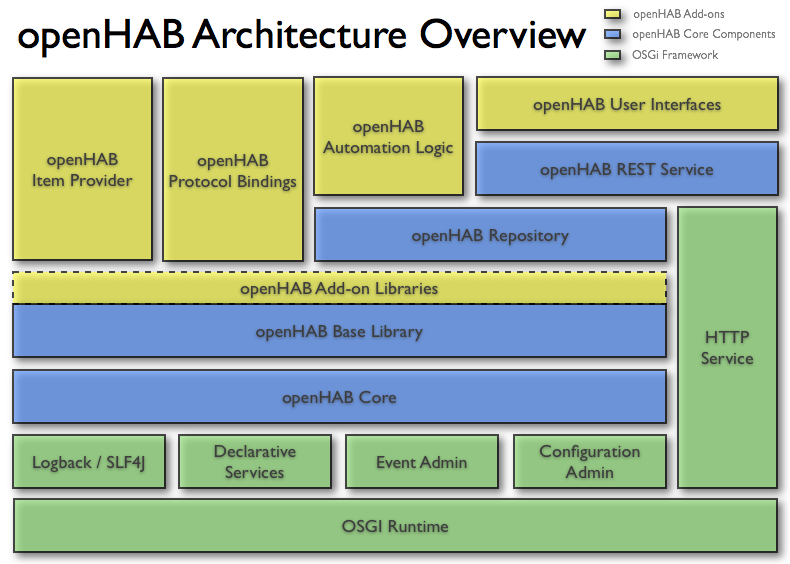
\includegraphics[scale=0.45]{report/img/openHAB_architecture}
	\caption{openHAB Architektur}
	\label{fig:ohArch}
\end{figure}

\subsubsection{Event Bus}
Der Basisservice von openHAB stellt der Event Bus dar. Über diesen Bus werden Events zwischen den verschiedenen OSGi Bundles gesendet. Die Events sind entweder Commands, welche eine Aktion ausführen, oder Status-Updates, welche Zustandsänderungen der Sensoren/Aktoren beinhalten. \\
Durch den Einsatz dieses Event Bus wird die Kopplung reduziert und Add-ons können somit einfach ausgetauscht werden. \\
Intern wurde der Event Bus mit Hilfe des OSGi Event Admin umgesetzt. Durch den Event Admin wird es möglich, dass sich weitere OSGi Bundles (also openHAB Add-ons) im Event Bus einklinken können.

\subsubsection{Bindings}
Bindings sind Verbindungen zwischen openHAB und den externen Systemen und bilden die Grundlage zur Konnektivität. Dadurch muss für jede Technologie ein eigenes Binding geschrieben werden. Für viele Technologien sind Bindings vorhanden, die einzeln heruntergeladen und als «Add-on» installiert werden können. Falls eine Technologie noch nicht unterstützt wird, kann man das Binding dazu selbst programmieren. Die wesentliche Aufgabe besteht darin, sich einerseits mit dem externen Gerät zu verbinden, auf dem Event Bus zu lauschen und die ausgetauschten Daten miteinander kompatibel zu machen. \\
Alle momentan verfügbare Bindings sind unter folgendem Link zu finden: \url{https://github.com/openhab/openhab/wiki/Bindings}

\begin{figure}[H]
	\centering
		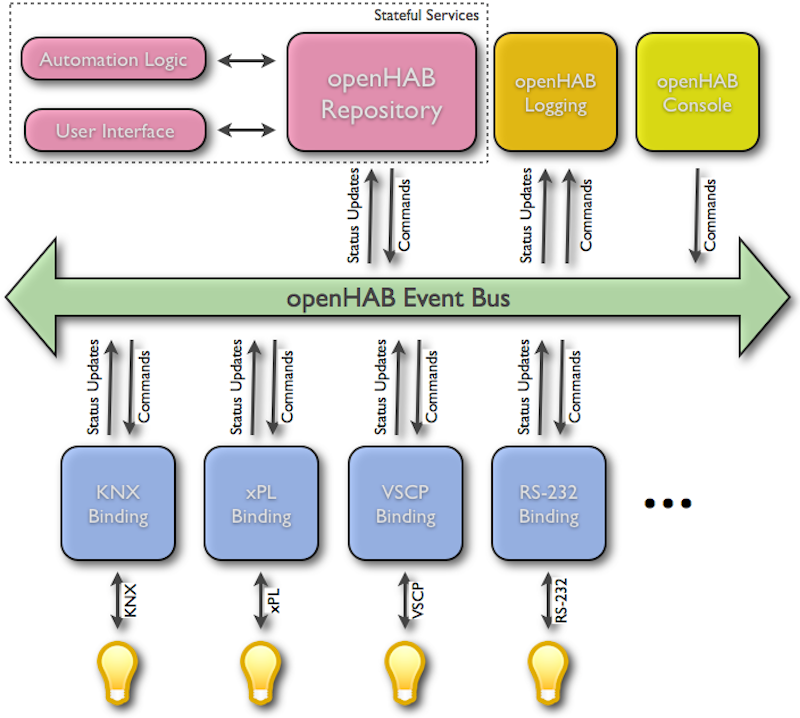
\includegraphics[scale=0.4]{report/img/communicationOH}
	\caption{Event Bus als Schnittstelle für Bindings}
	\label{fig:ohComm}
\end{figure}



\subsubsection{Items}
Wenn so viele unterschiedliche Technologien unterstützt und integriert werden sollen, dann stellt sich die Frage nach dem gemeinsamen Nenner bzw. einer einheitlichen internen Repräsentation. Aus diesem Grund wurden «Items» eingeführt, die zentrale Entität im openHAB Domainmodell. Alle Bindings implementieren ein Mapping zwischen den Daten des Sensors/Aktors und einem zugehörigen Item. Ein Item besteht aus:

\begin{itemize}
	\item Typ
	\item Name
	\item Formatierung
	\item Icon
	\item Gruppe
	\item Bindingparameter
\end{itemize}

Die Eigenschaften Typ und Name sind zwingend, die Anderen sind optional. Der Typ ist auf eine vorgegebene Auswahl beschränkt, der Name dient als Identifier und muss eindeutig sein.\\
\\
Je nach gewähltem Typ können Items die unterschiedlichsten Dinge repräsentieren. Ein sehr häufig verwendeter Typ ist das SwitchItem mit den beiden möglichen Werten ON und OFF. Dieses Item eignet sich aufgrund seines Wertebereichs hervorragend als Boolean. Ein SwitchItem kann stellvertretend für etwas reales, wie eine Lampe, oder für etwas abstraktes wie die Anwesenheit eines Bewohners stehen. Es ist wichtig zu verstehen, dass ein Item rein virtuell ist. Die Brücke zur echten Hardware wird erst über Bindingparameter geschlagen, denn dann verknüpft openHAB das Item mit dem entsprechenden Binding. Da die Bindingparameter eines Items aber optional sind macht openHAB keinen Unterschied zwischen virtuellen und realen Items.


\subsubsection{Item Repository}
Der Zustand eines Items muss die Ausführungsdauer einer openHAB Instanz überleben können, beispielsweise nach einem Neustart. Der Zustand muss ausserdem jederzeit abfragbar sein, egal ob sich der Zustand des Items gerade erst durch ein Event geändert hat oder schon über mehrere Startvorgänge hinweg genau so exisitiert. Diese Verantwortung übernimmt das Item Repository, welches permanent den Event Bus auf Status-Updates abhört und die Änderungen persistiert.

\subsubsection{Rules}
Rules sind die Werkzeuge zur Automatisierung. Dank einer Java-ähnlichen DSL können Aktionen ausgelöst werden, wenn gewisse Bedingungen erfüllt wurden. Das können einerseits Zustandsänderungen von Items, aber auch Systemevents oder Events von selbst angelegten Timern sein. 

\subsubsection{Sitemaps}
Sitemaps sind Konfigurationsfiles zur deklarativen Definition von User Interfaces. Sitemaps werden ebenfalls in einer Xtext basierten DSL geschrieben und haben eine baumartige Struktur. OpenHAB liest das Konfigurationsfile und stellt die Sitemap über eine REST API zur Verfügung. Eine mitgelieferte Webapplikation stellt das User Interface anschliessend im Browser dar. Layouttechnisch orientiert sich die Webapplikation am iOS 6 Design mit Listendarstellung und Drill-Down Prinzip. Die nativen iOS und Android Apps von openHAB verfolgen das selbe Bedienkonzept.\\
Die verschiedenen Elemente, die in Sitemaps verfügbar sind, können Items direkt über deren Name referenzieren. Einige Elemente sind dynamisch und erlauben eine werteabhängige Darstellung.

\subsection{Android App}
Als User Interface für unser System dient eine Android App. Zwar existieren bereits verschiedene openHAB Clients, sowohl als Web-App als auch als Android App, jedoch sind diese zu generisch. Man könnte argumentieren, dass es doch gut ist, wenn die App universell einsetzbar ist und oft hätte man damit recht. In unserem speziellen Szenario «Einbruchschutz» müssten wir aber zu viele Kompromisse eingehen. Deshalb haben wir uns dazu entschieden, die Android App selbst zu programmieren. 
\\ \\
Jede openHAB Installation bietet eine offene REST-Schnittstelle an, damit auch Clients von Drittanbietern auf Items und Sitemaps zugreifen können. Der openHAB Server ermöglicht sowohl das explizite Abfragen der Daten, als auch den umgekehrten Weg um Clients proaktiv über Änderungen zu informieren. 

\subsubsection{Features}
Die Features unserer App orientieren sich an den funktionalen Anforderungen zum Lösungsteil.

\begin{figure}[H]
	\centering
		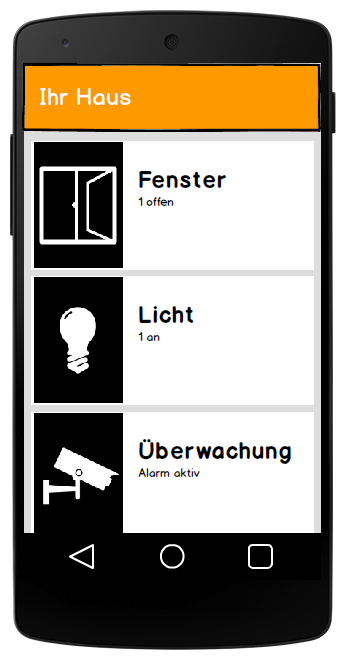
\includegraphics[scale=0.3]{report/img/mockup_overview.png}
	\caption{In dieser Ansicht soll der Benutzer möglichst auf einen Blick alle relevanten Informationen zum Sicherheitszustand seines Zuhauses erhalten. Von hier aus gelangt man zu den Bereichen «Fenster», «Licht» und «Überwachung». Für alle Bereiche wird eine kleine Zusammenfassung zum Status angezeigt.}
	\label{fig:mockupOverview}
\end{figure}

\begin{figure}[H]
	\centering
		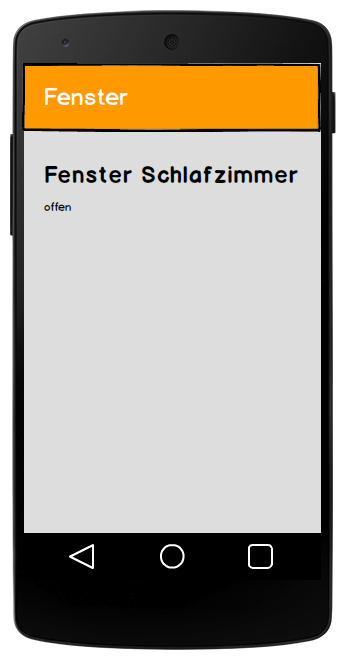
\includegraphics[scale=0.3]{report/img/mockup_window.png}
	\caption{Dieser Bereich zeigt alle Fenster, die mit einem Kontaktsensor ausgerüstet sind.}
	\label{fig:mockupWindow}
\end{figure}

\begin{figure}[H]
	\centering
		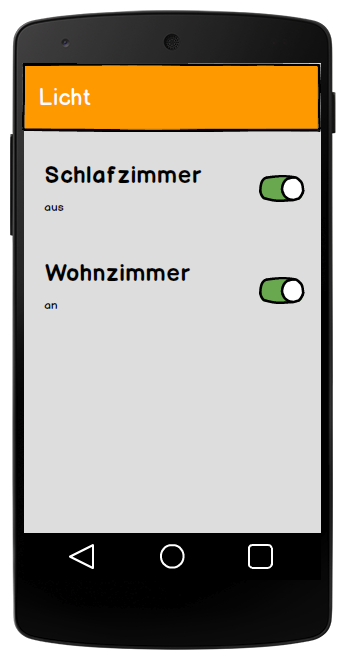
\includegraphics[scale=0.3]{report/img/mockup_light.png}
	\caption{Auf dieser Seite sind alle Lampen aufgelistet, die in openHAB integriert wurden. Mit einem Switch können diese ein- oder ausgeschaltet werden.}
	\label{fig:mockupLight}
\end{figure}


\subsection{Anbindung Cloud}

In den funktionalen Anforderungen zum Basisszenario wurde festgelegt, dass Geschehnisse auf dem lokalen Bus (openHAB) an die Cloud gesendet werden müssen. Als Cloud-Plattform wurde Microsoft Azure bereits zu Beginn der Arbeit definiert. Damit die Daten von openHAB in die Cloud gelangen gibt es im Wesentlichen zwei Möglichkeiten: Entweder man entwickelt selbst ein Plugin für openHAB oder man verwendet das openHAB MQTT Persistence Plugin. MQTT ist ein Publish/Subscribe Protokoll und besonders gut für IOT Systeme mit langsamer oder instabiler Internetverbindung geeignet. Wir haben uns für die Variante mit MQTT entschieden. OpenHAB fungiert als MQTT-Client und kann so konfiguriert werden, dass Events auf dem Bus automatisch an einen MQTT-Broker gesendet werden, der von uns auf Microsoft Azure installiert wurde. Um die Daten zu verarbeiten muss ein MQTT-Client auf Microsoft Azure laufen und die Nachrichten vom Broker entgegennehmen. Danach steht uns frei, wie die Daten verarbeitet werden.

\subsubsection{MQTT Broker Evaluation}
Für die Evaluation des Brokers haben wir eine List mit unseren Anforderungen erstellt: 

\begin{enumerate}
	\item Open Source/Freeware
	\item SSL TLS Verschlüsselung
	\item Benutzername \& Passwort Authentifizierung
	\item High throughput, Low latency
	\item Cloud Ready
	\item Einfache Installation
	\item Qualit of Service Level: Exactly once
	\item Last Will unterstützung (Message, die gesendet wird, wenn der Client die Verbindung schliesst)
\end{enumerate}

\textbf{HiveMQ (\url{http://www.hivemq.com})} \\
HiveMQ ist ein proprietärer MQTT-Broker und erfüllt alle unsere Kriterien bis auf das erste Kriterium. Jeder Gebrauch des Brokers muss bezahlt werden, siehe: \url{http://www.hivemq.com/pricing/}.

\textbf{Mosquitto (\url{http://eclipse.org/mosquitto/})}\\
Mosquitto ist ein Open Source Broker, dessen Projekt von Roger Light im Jahr 2010 auf die Beine gestellt wurde. Seit der Version 1.4 läuft das Projekt unter der Eclipse Foundation. \\
Die aktuelle Implementation benötigt lediglich 120kB Speicherplatz und 3MB RAM bei 1000 verbundenen Clients. Ein Belastungstest von 100'000 Clients erzielte erfolgreiche und zufriedenstellende Resultate.
Alle anderen Kriterien werden ebenfalls erfüllt.

\textbf{CloudMQTT} \\
CloudMQTT unterscheidet sich von den anderen Brokern, da dieser nicht selbst betrieben werden kann. Das bedeutet, man erstellt bei CloudMQTT eine Instanz und kann denn neu erstellten Broke über verschiedene APIs ansteuern. \\
Der Anbieter stellt verschiedene Preispläne zur Verfügung (\url{http://www.cloudmqtt.com/plans.html}). Ab 10 Verbindungen bzw. 10Kbit/s Bandbreite muss für die Leistung bezahlt werden. \\
Ob TLS SSL Verschlüsselung unterstützt wird, ist in der spärlichen Dokumentation nicht ersichtlich.

\textbf{Fazit} \\
Aufgrund der gesammelten Daten der drei Produkte wurde entschieden, Mosquitto einzusetzen. Es ist das einzige Produkt, welches alle unsere Kriterien erfüllt. Da dieses Projekt durch die Eclipse Foundation unterstützt wird, besteht die Hoffung, dass die Zusammenarbeit mit openHAB unterstützt bzw. miteinbezogen wurde.

\subsubsection{Client-Library}
In unserem Systemaufbau wird es zwei MQTT-Clients geben. Einerseits durch das openHAB-Binding, da die Events auf dem EventBus über MQTT in die Azure Cloud gesendet werden soll. Andererseits wird in der Cloud eine Worker Role diese Events konsumieren und persistieren. \\
Das Binding von openHAB besteht bereits, daher muss nur noch eine Client-Implementation für C\# gesuchtwerden. Nach kurzer Rechereche scheint die «M2Mqtt» Library sehr verbreitet zu sein. \\
Durch aufsetzen eines Prototyps konnte die benötigte Funktionalität erfasst werden. Sie erfüllt alle Kriterien, die auch an den Broker gestellt wurden.

\subsection{Notification}
Damit ein Sicherheitssystem Sinn macht, muss der Besitzer benachrichtigt werden, sobald sich ein Zustand der Sensoren ändert. Genauer gesagt soll der Benutzer informiert werden, wenn der Bewegungsmelder oder der Fensterkontakt im Alarm-Modus eine Veränderung registriert. Ansonsten müsste der Benutzer permanent die Status im Android-App überwachen. Für die Umsetzung bietet sich der Google Cloud Message Dienst (GCM) an, der auch von Microsoft empfohlen wird. Da nur die Android-Platform unterstützt werden muss, wird auf den Einsatz des Azure Notification Hubs verzichtet und die direkte Verbindung zum GCM-Dienst gesucht.

\subsection{Sicherheit}
In unserem Szenario, Einbruchschutz, ist das Thema Sicherheit sehr wichtig. Daher lohnt es sich dazu  Gedanken zu machen. Man kann das System grob in drei Bereiche einteilen, an denen ein Angriff angesetzt werden kann:
\begin{itemize}
	\item Cloud
	\item Android App
	\item Systemaufbau mit Sensoren/Aktoren
	\item Kommunikation der HomeMatic Komponenten
\end{itemize}

\subsubsection{Cloud}
Die Angriffsfläche in der Cloud ist ziemlich eingeschränkt. Sicherheitsrelevante Aspekte sind der Broker und die persistierten Daten im Storage. Zugriff auf diese Ressourcen erhält man über verschiedene Wege. Einerseits über das Management Web-Interface von Microsoft Azure oder über ein Connection-String. Durch die Verwendung eines Connection Strings für den Verbindungsaufbau zum Storage kein Benutzername bzw. Passwort mitgegeben werden.

Zugriff auf diese Ressourcen haben nur authorisierte Personen die ein entsprechendes Microsoft Konto besitzen und auf die Subscription zugelassen werden. Eine vernünftige Attack kann daher nur durch das Hijacken eines Accounts gefahren werden. Als Gegenmassnahme müssen ausreichend sichere Passwörter auf den persönlichen Konten gesetzt werden. Das liegt in der Verantwortung der einzelnen Personen, die auf diese Subscription Zugriff besitzen.

Auf den Storage kann ausser der Management-Oberfläche auch über ein Connection-String zugegriffen werden. Dieser String kann nur über die Management-Oberfläche eingesehen werden und ist daher sicher versteckt. Weiter könnte der Connection String aus dem Source-Code der Worker Role gelesen werden, da er dort für den Verbindungsaufbau zum Storage verwendet wird. Diese Worker Role und deren Source-Code befindet sich innerhalb der Cloud und ist somit auch gegen ein Eindringen gesichert. \\

\subsubsection{Android App}
Über das Android App kann das ganze System manipuliert werden. Daher stellt dies ein grosses Sicherheits-Risiko dar. Gesichtert wird das App durch Eingabe von Benutzerdaten, um auf die RESTful-API des openHAB zuzugreifen. \\
Auch hier wird die Person, die das App verwendet zur Verantwortung gezogen, um das Smartphone durch ein sicheres Passwort zu schützen.

\subsubsection{Systemaufbau mit Sensoren/Aktoren}
Wenn sich die angreifende Person bereits im Haus befindet,hat sie die entsprechenden Alarme bereits ausgelöst und wurde durch die Webcam aufgenommen. \\
Für dieses Szenario ist das grösste Risiko, dass die Person die Videoüberwachung bemerkt und aus diesem Grund das Raspberry Pi zerstört bzw. mitnimmt. Um die aufgezeichneten Daten zu sichern, werden die von der Kamera erzeugten Bilder über MQTT im Cloud-Storage abgelegt. Auch wenn das Raspberry Pi zerstört wird, sind die Bilder nun gesichert und können im Nachhinein vom Storage heruntergeladen werden.

\subsubsection{HomeMatic Kommunikation}
Da die HomeMatic Komponenten untereinander drahtlos kommunizieren besteht hier ebenfalls die Gefahr einer Attacke. HomeMatic setzt für die Übertragung auf den Funkstandard BidCos. Diese Standard sieht vor, dass das 868 MHz Band verwendet wird. Im Vergleich zu 2.4 GHz besitzt man so eine grösse Reichweite und die Gefahr von Interferenz durch andere Funkgeräte ist sehr minim.\\
Bezüglich Sicherheit sieht der Standard lediglich vor, die übertragenen Daten durch XOR-Operationen unleserlich zu machen. HomeMatic hat daher bei der Implentierung dieses Stanards die Verschlüsselung durch AES-128 verstärkt. Der zur Verschlüsselung verwendete Key ist in der Zentrale hinterlegt und kann bei Bedarf geändert werden.


\subsubsection{Fazit}
Wie aus den Ausführungen zur Sicherheit ersichtlich ist, können alle technischen Sicherheits-Risiken abgedeckt werden. Die grösste Schwachstellt ist jeweils der Mensch, der durch Social-Engineering-Techniken manipuliert werden kann und so Zugriff auf das Android App gewährt.

\subsection{Allgemeine Systemsicht}
Anhand der Problembeschreibung wurde ein Plan erarbeitet, der das ganze System verständlich beschreibt. Abbildung \ref{fig:systemView} stellt die wichtigsten Komponenten und Entitäten aus der Problemdomäne in gegenseitiger Beziehung dar.

\begin{figure}[h!]
	\centering
		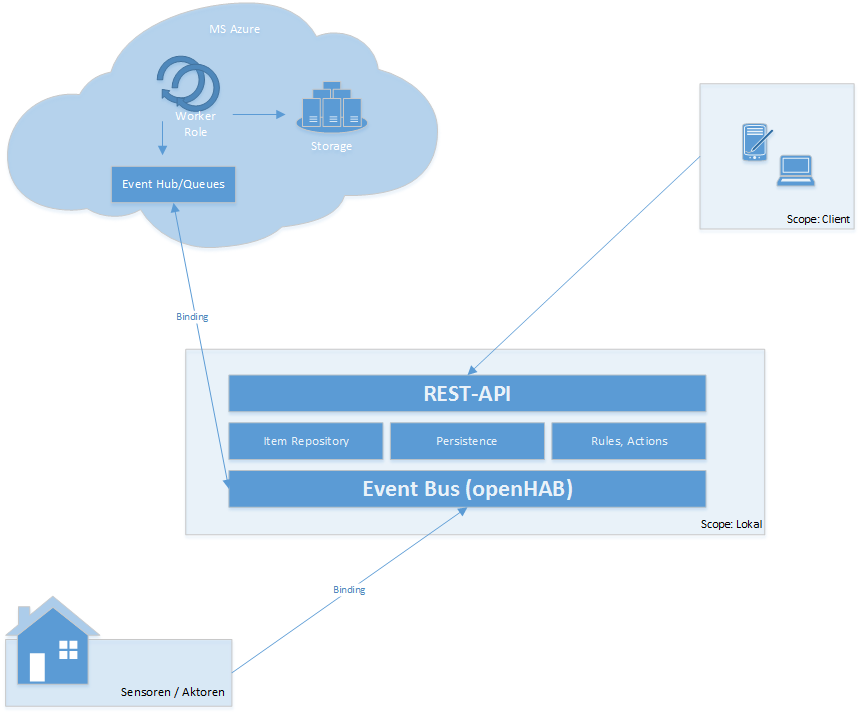
\includegraphics[scale=0.55]{report/img/systemuebersicht}
	\caption{Systemübersicht}
	\label{fig:systemView}
\end{figure}

\pagebreak